\documentclass[letterpaper,10pt]{article}

\usepackage{enumitem}
\usepackage{titling}
\usepackage{listings,listings-rust}
\usepackage{url}
\usepackage{soul}
\usepackage{hyperref}
\usepackage{setspace}
\usepackage{subfig}
\usepackage{sectsty}
\usepackage{pdfpages}
\usepackage{colortbl}
\usepackage{multirow}
\usepackage{multicol}
\usepackage{relsize}
\usepackage{amsmath}
\usepackage{wasysym}
\usepackage{fancyvrb}
\usepackage[yyyymmdd]{datetime}
\usepackage{amsmath,amssymb,amsthm,graphicx,xspace}
\usepackage[titlenotnumbered,noend,noline]{algorithm2e}
\usepackage[compact]{titlesec}
\usepackage{XCharter}
\usepackage[T1]{fontenc}
\usepackage[scaled]{beramono}
\usepackage[normalem]{ulem}
\usepackage{booktabs}
\usepackage{tikz}
\usetikzlibrary{arrows.meta,automata,shapes,trees,matrix,chains,scopes,positioning,calc,decorations.pathreplacing}
\tikzstyle{block} = [rectangle, draw, fill=blue!20, 
    text width=2.5em, text centered, rounded corners, minimum height=2em]
\tikzstyle{bw} = [rectangle, draw, fill=blue!20, 
    text width=4em, text centered, rounded corners, minimum height=2em]

\definecolor{namerow}{cmyk}{.40,.40,.40,.40}
\definecolor{namecol}{cmyk}{.40,.40,.40,.40}
\renewcommand{\dateseparator}{-}

\let\LaTeXtitle\title
\renewcommand{\title}[1]{\LaTeXtitle{\textsf{#1}}}

\lstset{basicstyle=\footnotesize\ttfamily,breaklines=true}

\newcommand{\CPP}{C\nolinebreak\hspace{-.05em}\raisebox{.4ex}{\tiny\bf +}\nolinebreak\hspace{-.10em}\raisebox{.4ex}{\tiny\bf +}}
\def\CPP{{C\nolinebreak[4]\hspace{-.05em}\raisebox{.4ex}{\tiny\bf ++}}}

\newcommand{\handout}[5]{
  \noindent
  \begin{center}
  \framebox{
    \vbox{
      \hbox to 5.78in { {\bf ECE459: Programming for Performance } \hfill #2 }
      \vspace{4mm}
      \hbox to 5.78in { {\Large \hfill #4  \hfill} }
      \vspace{2mm}
      \hbox to 5.78in { {\em #3 \hfill \today} }
    }
  }
  \end{center}
  \vspace*{4mm}
}

\newcommand{\lecture}[3]{\handout{#1}{#2}{#3}{Lecture#1}}
\newcommand{\tuple}[1]{\ensuremath{\left\langle #1 \right\rangle}\xspace}

\addtolength{\oddsidemargin}{-1.000in}
\addtolength{\evensidemargin}{-0.500in}
\addtolength{\textwidth}{2.0in}
\addtolength{\topmargin}{-1.000in}
\addtolength{\textheight}{1.75in}
\addtolength{\parskip}{\baselineskip}
\setlength{\parindent}{0in}
\renewcommand{\baselinestretch}{1.5}
\newcommand{\term}{Winter 2020}

\singlespace


\begin{document}

\lecture{3\footnote{version 2: removed undefined behaviour} --- Branch Prediction \& Amdahl's Law}{\term}{Patrick Lam \& Jeff Zarnett}

\section*{Branch Prediction and Misprediction}

The compiler (and the CPU) take a look at code that results in branch instructions  such as loops, conditionals, or the dreaded \texttt{goto}\footnote{Which I still maintain is a swear word in C.}, and it will take an assessment of what it thinks is likely to happen. By default I think it's assumed that backward branches are taken and forward branches are not taken (but that may be wrong).  Well, how did we get here anyway?

In the beginning the CPUs and compilers didn't really think about this sort of thing, they would just come across instructions one at a time and do them and that was that. If one of them required a branch, it was no real issue. Then we had pipelining: the CPU would fetch the next instruction while decoding the previous one, and while executing the instruction before. That means if evaluation of an instruction results in a branch, we might go somewhere else and therefore throw away the contents of the pipeline. Thus we'd have wasted some time and effort. If the pipeline is short, this is not very expensive. But pipelines keep getting longer\ldots

So then we got to the subject of branch prediction. The compiler and CPU look at instructions on their way to be executed and analyze whether it thinks it's likely the branch is taken. This can be based on several things, including the recent execution history. If we guess correctly, this is great, because it minimizes the cost of the branch. If we guess wrong, we have to flush the pipeline and take the performance penalty.

The compiler and CPU's branch prediction routines are pretty smart. Trying to outsmart them isn't necessarily a good idea. But we can give the compiler (\texttt{gcc} at least) some hints about what we think is likely to happen. Our tool for this is the \texttt{\_\_builtin\_expect()} function, which takes two arguments, the value to be tested and the expected result.

In the linux \texttt{compiler.h} header there are two neat little shortcuts defined:

\begin{lstlisting}[language=C]
# define likely(x)      __builtin_expect(!!(x), 1)
# define unlikely(x)    __builtin_expect(!!(x), 0)
\end{lstlisting}

These are nice ways of saying that we expect \texttt{x} to be true (likely) or false (unlikely). These hints tell the compiler some information about how it should predict. It will then arrange the instructions in such a way that, if the prediction is right, the instructions in the pipeline will be executed. But if we're wrong, then the instructions will have to be flushed.

Compile with at least optimization level 2 (\texttt{-O2}) for the compiler to take these hints. Otherwise they won't do anything. 

It takes a bit of trickery to force branch mispredicts. {\tt gcc} extensions allow hinting, but usually {\tt gcc} or the processor is smart enough to ignore bad hints. This code from~\cite{mispredict} worked in 2013, though:


\begin{lstlisting}[language=C]
        #include <stdlib.h>
        #include <stdio.h>

        static __attribute__ ((noinline)) int f(int a) { return a; }

        #define BSIZE 1000000
        int main(int argc, char* argv[]) 
        {
          int *p = calloc(BSIZE, sizeof(int));
          int j, k, m1 = 0, m2 = 0;
          for (j = 0; j < 1000; j++) {
            for (k = 0; k < BSIZE; k++) {
              if (__builtin_expect(p[k], EXPECT_RESULT)) {
                m1 = f(++m1);
              } else {
                m2 = f(++m2);
              }
            }
          }
          printf("%d, %d\n", m1, m2);
        }
\end{lstlisting}

Running it yielded:
\begin{lstlisting}[language=C]
plam@plym:~/459$ gcc -O2 likely-simplified.c -DEXPECT_RESULT=0 -o likely-simplified
plam@plym:~/459$ time ./likely-simplified
0, 1000000000

real	0m2.521s
user	0m2.496s
sys	0m0.000s
plam@plym:~/459$ gcc -O2 likely-simplified.c -DEXPECT_RESULT=1 -o likely-simplified
plam@plym:~/459$ time ./likely-simplified
0, 1000000000

real	0m3.938s
user	0m3.868ss
sys	0m0.000s
\end{lstlisting}
Some versions of {\tt gcc} and {\tt clang} seem to have gotten smart enough to reject bogus hints since then. In 2018, gcc 7.2.0 shows the same time on Linux 4.14.12 (post-mitigation) running on a Pentium G645, while clang 6.0.0 shows a difference of 2.46s vs 2.81s.

In the original source~\cite{mispredict} the author reports the following results: scanning a one million element array, with all elements initially zero, the results are:
\vspace*{-1em}
\begin{itemize}[noitemsep]
	\item No use of hints: \texttt{0:02.68 real,  2.67 user, 0.00 sys}
	\item Good prediction: \texttt{0:02.28 real,  2.28 user, 0.00 sys}
	\item Bad prediction: \texttt{0:04.19 real,  4.18 user, 0.00 sys}
\end{itemize}

\paragraph{Using the hints.} From these results we can see pretty clearly that if we're wrong, the penalty can be pretty large (assuming the compiler does not look at your hint and think ``stupid human, I know better''). Under a lot of circumstances then, it's probably best just to leave it alone, unless we're really, really, really sure. 

How sure do we have to be? The answer depends dramatically on the code, the CPU you're using, the compiler, and all those little details. But~\cite{mispredict} to the rescue here again, because there are some tests here. To cut to the chase, when about one in ten thousand values in the array is nonzero, then it's roughly the ``break-even'' point for the setup as described.

Conclusion: it's hard to outsmart the compiler. Maybe it's better not to try.

\section*{How does branch prediction work, anyway?}
We can write software. The hardware will make it fast. If we understand the hardware, we can understand when it has trouble making our software fast.

You've seen how branch prediction works in ECE 222. However, we'll talk about it today in the context of performance. Notes based on a transcript of a talk by Dan Luu~\cite{branchprediction}.

I want you to pick up two points from this discussion:
\vspace*{-1em}
\begin{itemize}[noitemsep]
\item how branch predictors work---this helps you understand some of the apparent randomness in your
execution times, and possibly helps you make your code more predictable; and,
\item applying a (straightforward) expected value computation to predict performance.
\end{itemize}

Let's consider the following assembly code:

\hspace*{2em} \begin{minipage}{.4\textwidth} \begin{lstlisting}
branch_if_not_equal x, 0, else_label
// Do stuff
goto end_label
else_label:
// Do things
end_label:
// whatever happens later
\end{lstlisting}
\end{minipage}

The {\tt branch} instruction may be followed by either ``stuff'' or ``things''.
The pipeline needs to know what the next instruction is, for instance to fetch it.
But it can't know the next instruction until it almost finishes executing the branch.
Let's look at some pictures, assuming a 2-stage pipeline.

With no prediction, we need to serialize:

\begin{center}
\begin{tabular}{c|c|c|c}
bne.1 & bne.2 \\ \hline
& & things.1 & things.2
\end{tabular}
\end{center}

\begin{minipage}{.49\textwidth}
Let's predict that ``things'' gets taken.
If our prediction is correct, we save time.

\begin{center}
\begin{tabular}{c|c|c}
bne.1 & bne.2 \\ \hline
& things.1 & things.2 \\
\\
\end{tabular}
\end{center}
\end{minipage} \hspace*{.02\textwidth} \begin{minipage}{.49\textwidth}
But we might be wrong and need to throw out the bad prediction.

\begin{center}
\begin{tabular}{c|c|c|c}
bne.1 & bne.2 \\ \cline{1-2}
& \sout{things.1} \\ \hline
& & stuff.1 & stuff.2
\end{tabular}
\end{center}
\end{minipage}

\paragraph{Cartoon model.} We need to quantify the performance.
For the purpose of this lecture, let's pretend that our pipelined
CPU executes, on average, one instruction per clock;
mispredicted branches cost 20 cycles, while correctly-predicted
branches cost 1 cycle. We'll also assume that the instruction
mix contains 80\% non-branches and 20\% branches. So we can predict
average cycles per instruction.

With no prediction (or always-wrong prediction):
\[
\mathrm{non\_branch\_\%} \times 1 \mathrm{~cycle} + \mathrm{branch\_\%} \times 20 \mathrm{~cycles} = 4.8 \mathrm{~cycles}.
\]
With perfect branch prediction:
\[
\mathrm{non\_branch\_\%} \times 1 \mathrm{~cycle} + \mathrm{branch\_\%} \times 1 \mathrm{~cycle} = 1 \mathrm{~cycle}.
\]
So we can make our code run 4.8$\times$ faster with branch prediction!

\paragraph{Predict taken.} What's the simplest possible thing? We can
predict that a branch is always taken. (Loop branches, for instance,
account for many of the branches in an execution, and are often taken.)
If we got 70\% accuracy, then our cycles per instruction would be:
\[
(0.8 + 0.7 \times 0.2) \times 1 \mathrm{~cycle} + (0.3 \times 0.2) \times 20 \mathrm{~cycles} = 2.14 \mathrm{~cycles}.
\]
The simplest possible thing already greatly improves the CPU's average throughput.

\paragraph{Backwards taken, forwards not taken (BTFNT).}
Let's leverage that observation about loop branches to do better.
Loop branches are, by definition, backwards (go back to previous
code). So we can design a branch predictor which predicts ``taken''
for backwards and ``not taken'' for forwards. The compiler can then
use this information to encode what it thinks about forwards branches
(that is, making the not-taken branch the one it thinks is more likely).
Let's say that this might get us to 80\% accuracy. \[
(0.8 + 0.8 \times 0.2) \times 1 \mathrm{~cycle} + (0.2 \times 0.2) \times 20 \mathrm{~cycles} = 1.76 \mathrm{~cycles}.
\]
The PPC 601 (1993) and 603 used this scheme.

\paragraph{Going dynamic: using history for branch prediction.}
So far, we will always make the same prediction at each branch---known as a
\emph{static} scheme. But we can do better by using what recently happened to
improve our predictions. This is particularly important when program execution
contains distinct phases, with distinct behaviours.
We therefore move to \emph{dynamic} schemes.

Once again, let's start with the simplest possible thing. For every branch,
we record whether it was taken or not last time it executed (a 1-bit scheme).
Of course, we can't store all branches. So let's use the low 6 bits of the address
to identify branches. Doing so raises the prospect of \emph{aliasing}:
different branches (with different behaviour) map to the same spot in the table.

We might get 85\% accuracy with such a scheme.
\[
(0.8 + 0.85 \times 0.2) \times 1 \mathrm{~cycle} + (0.15 \times 0.2) \times 20 \mathrm{~cycles} = 1.57 \mathrm{~cycles}.
\]

At the cost of more hardware, we get noticeable performance improvements. The DEC EV4 (1992) and
MIPS R8000 (1994) used this one-bit scheme.

\paragraph{Two-bit schemes.}
What if a branch is almost always taken but occasionally not taken (e.g. TTTTTTNTTTT)?
We get penalized twice
for that misprediction: once when we mispredict the not taken, and once when we mispredict the
next taken. So, let's store whether a branch is ``usually'' taken, using a so-called
2-bit saturating counter.

Every time we see a taken branch, we increment the counter for that
branch; every time we see a not-taken branch, we decrement. Saturating
means that we don't overflow or underflow. We instead stay at 11 or
00, respectively.

If the counter is 00 or 01, we predict ``not taken''; if it is 10 or
11, we predict ``taken''.

With a two-bit counter, we can have fewer entries at the same size, but they'll do better.
It would be reasonable to expect 90\% accuracy.
\[
(0.8 + 0.9 \times 0.2) \times 1 \mathrm{~cycle} + (0.1 \times 0.2) \times 20 \mathrm{~cycles} = 1.38 \mathrm{~cycles}.
\]

This was used in a number of chips, from the LLNL S-1 (1977) through the Intel Pentium (1993).

\paragraph{Two-level adaptive, global.}
We're still not taking patterns into account. Consider the following {\tt for} loop.
\begin{lstlisting}[language=C]
for (int i = 0; i < 3; ++i) {
  // code
}
\end{lstlisting}
The last three executions of the branch determine the next direction:
\begin{verbatim}
 TTT => N
 TTN => T
 TNT => T
 NTT => T
\end{verbatim}
Let's store what happened the last few times we were at a particular address---the
\emph{branch history}. From a branch address and history, we derive an index, which
points to a table of 2-bit saturating counters. What's changed from the two-bit scheme
is that the history helps determine the index and hence the prediction.

After we take a branch, we add its direction to the history, so that the next lookup
maps to a different table entry.

This scheme might give something like 93\% accuracy.
\[
(0.8 + 0.93 \times 0.2) \times 1 \mathrm{~cycle} + (0.07 \times 0.2) \times 20 \mathrm{~cycles} = 1.27 \mathrm{~cycles}.
\]

The Pentium MMX (1996) used a 4-bit global branch history.

\paragraph{Two-level adaptive, local.}
The change here is that the CPU keeps a separate history for each branch.
So the branch address determines which branch history gets used.
We concatenate the address and history to get the index, which then points to a
2-bit counter again. We are starting to encounter diminishing returns, but we might
get 94\% accuracy:
\[
(0.8 + 0.94 \times 0.2) \times 1 \mathrm{~cycle} + (0.06 \times 0.2) \times 20 \mathrm{~cycles} = 1.23 \mathrm{~cycles}.
\]

The Pentium Pro (1996), Pentium II (1997) and Pentium III (1999) use this.

\paragraph{gshare.}
Instead of concatenating the address and history, we can xor them. This allows
us to use more bits for both the history and address. This keeps the accuracy the same,
but simplifies the design.

\paragraph{Other predictors.} We can build (and people have built) more sophisticated predictors.
These predictors could, for instance, better handle aliasing, where
different branches/histories map to the same index in the table. But we'll stop here.

\paragraph{Summary of branch prediction.} We can summarize as follows.
Branch prediction enables pipelining and hence increased performance.
We can create a model to estimate just how critical branch prediction
is for modern processors. Fortunately, most branches are predictable
now. Aliasing (multiple branches mapping to the same entry in a
prediction table) can be a problem, but processors are pretty good at
dealing with that too.

\section*{Cache side-channel attacks}

In early 2018, the Spectre~\cite{Kocher2018spectre} and Meltdown~\cite{Lipp2018meltdown} attacks were disclosed. These attacks leverage performance features of modern CPUs to break process isolation guarantees---in principle, a process shouldn't be able to read memory that belongs to the kernel or to other processes.

The concept of cache side-channel attacks has been known for a while. If an attacker can get some memory loaded into the cache, then it can extract that memory using a cache side-channel attack.

Spectre and Meltdown can cause privileged memory to be loaded into the cache, and then extracted using a cache side-channel attack. We'll talk about Spectre (variant 2), since it attacks branch prediction in particular. My explanation follows~\cite{masters18:_what_meltd_spect} by Jon Masters of RedHat. However, you should now have enough background to follow the Google Project Zero description at~\cite{horn18:_readin}.

We know that at a branch, the CPU will start speculatively executing code at the inferred target of the branch. To exploit this vulnerability, the attack code convinces the CPU to speculatively execute code of its choice. The speculatively-executed attack code reads secret data (e.g. from the hypervisor kernel) and puts it in the cache. Once the data is in the cache, the attack proceeds by extracting the data from the cache.
\newpage

\section*{Limits to parallelization}
I mentioned briefly in Lecture 1 that programs often have a sequential
part and a parallel part. We'll quantify this observation today
and discuss its consequences.

\paragraph{Amdahl's Law.} One classic model of parallel execution
is Amdahl's Law. In 1967, Gene Amdahl argued that improvements in
processor design for single processors would be more effective than
designing multi-processor systems. Here's the argument. Let's say that
you are trying to run a task which has a serial part, taking fraction 
$S$, and a parallelizable part, taking fraction $P = 1-S$. Define $T_s$
to be the total 
amount of time needed on a single-processor system.
Now, moving to a parallel system with $N$ processors, the parallel
time $T_p$ is instead:
\[ T_p = T_s \cdot (S + \frac{P}{N}). \]
{\bf As $N$ increases, $T_p$ is dominated by $S$, limiting potential
speedup.}

We can restate this law in terms of speedup, which is the 
original time $T_s$ divided by the sped-up time $T_p$:
\[ \mbox{speedup} = \frac{T_s}{T_p} = \frac{1}{S+P/N}. \]
Replacing $S$ with $(1-P)$, we get:
\[ \mbox{speedup} = \frac{1}{(1-P)+P/N}, \]
and
\[ \mbox{max speedup} = \frac{1}{(1-P)}, \]
since $\frac{P}{N} \rightarrow 0$.

\paragraph{Plugging in numbers.} If $P = 1$, then we can indeed get good
scaling; running on an $N$-processor machine will give you a speedup
of $N$. Unfortunately, usually $P < 1$.  Let's see what happens.

\begin{center}
\begin{tabular}{r|r}
$P$ & speedup ($N=18$) \\ \hline
1 & 18 \\
0.99 & $\sim$ 15 \\
0.95 & $\sim$ 10 \\
0.5 & $\sim$ 2
\end{tabular}
\end{center}
Graphically, we have something like this:
\begin{center}
  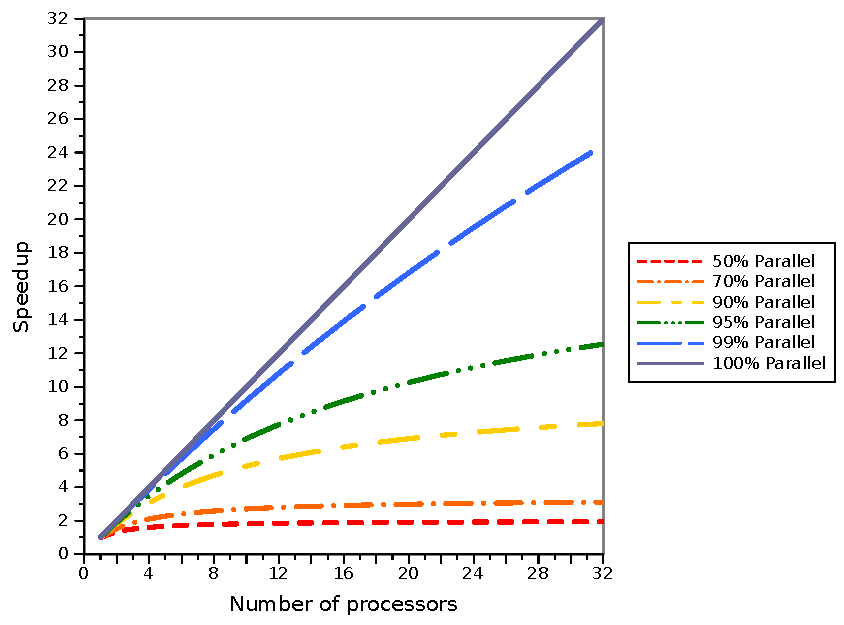
\includegraphics[width=0.5\textwidth]{images/parallel-scaling}
\end{center}


Amdahl's Law tells you how many cores you can hope to leverage in an
execution given a fixed problem size, if you can estimate $P$.

Let us consider an example from~\cite{mte241}: Suppose we have a task that can be executed in 5~s and this task contains a loop that can be parallelized. Let us also say initialization and recombination code in this routine requires 400~ms. So with one processor executing, it would take about 4.6~s to execute the loop. If we split it up and execute on two processors it will take about 2.3~s to execute the loop. Add to that the setup and cleanup time of 0.4~s and we get a total time of 2.7~s. Completing the task in 2.7~s rather than 5~s represents a speedup of about~46\%. Applying the formula, we get the following run times:

\begin{center}
	\begin{tabular}{l|l}
	\textbf{Processors} & \textbf{Run Time (s)} \\ \hline
	1 & 5\\
	2 & 2.7\\
	4 & 1.55\\
	8 & 0.975\\
	16 & 0.6875 \\
	32 & 0.54375 \\
	64 & 0.471875 \\
	128 & 0.4359375\\
	\end{tabular}
\end{center}

   \paragraph{Empirically estimating parallel speedup $P$.}
Assuming that you know things that are actually really hard to know, here's a formula for estimating speedup. You don't have to commit it to memory:
  \[P_{\mbox{\scriptsize estimated}} = \frac{\frac{1}{\mbox{\em speedup}}-1}{\frac{1}{N}-1}.\]

It's just an estimation, but you can use it to guess the fraction of parallel code, given $N$ and the speedup. You can then use $P_{\mbox{\scriptsize estimated}}$ to predict speedup for a different number of processors.

\paragraph{Consequences of Amdahl's Law.}
For over 30 years, most performance gains did indeed come from
increasing single-processor performance. The main reason that we're
here today is that, as we saw last time,
single-processor performance gains have hit the wall.

By the way, note that we didn't talk about the cost of synchronization
between threads here. That can drag the performance down even more.

\paragraph{Amdahl's Assumptions.}
Despite Amdahl's pessimism, we still all have multicore computers today.
Why is that? Amdahl's Law assumes that:
\begin{itemize}[noitemsep]
    \item problem size is fixed (read on);
    \item the program, or the underlying implementation, behaves the same on 1 processor as on $N$ processors; and
    \item that we can accurately measure runtimes---i.e. that overheads don't matter.
\end{itemize}

% replace Amdahl's law with how branch predictors work
%% \paragraph{Generalizing Amdahl's Law.} We made a simplification,
%% which was that programs only have one parallel part and one serial part.
%% Of course, this is not true. The program may have many parts,
%% each of which we can tune to a different degree.

%% Let's generalize Amdahl's Law:

%% \begin{itemize}
%% \item  $f_1, f_2, \ldots, f_n$: fraction of time in part $n$
%% \item  $S_{f_1}, S_{f_n}, \ldots, S_{f_n}$: speedup for part $n$
%% \end{itemize}

%% Then,
%% \[\mbox{\em speedup} = \frac{1}{\frac{f_1}{S_{f_1}} + \frac{f_2}{S_{f_2}} + \ldots +
%%     \frac{f_n}{S_{f_n}}}.\]

%% \paragraph{Example.} Consider a program with 4 parts in the following scenario:

%% \begin{center}
%%     \begin{tabular}{r|r|r|r}
%%     \multicolumn{2}{l}{} & \multicolumn{2}{|c}{Speedup} \\
%%     Part & Fraction of Runtime & Option 1 & Option 2\\
%%     \hline
%%     1 & 0.55 & 1  & 2\\
%%     2 & 0.25 & 5  & 1\\
%%     3 & 0.15 & 3  & 1\\
%%     4 & 0.05  & 10 & 1\\
%%     \end{tabular}
%% \end{center}

%%     (Note: these speedups don't have to be speedups from parallelization.)
    
%%   We can implement either Option 1 or Option 2. 
%%   Which option is better?

%%   ``Plug and chug'' the numbers:
%% \begin{itemize}
%% \item  {\bf Option 1.}

%%   \[ \mbox{\em speedup} = \frac{1}{0.55 + \frac{0.25}{5} + \frac{0.15}{3} + \frac{0.05}{5}}
%%     = 1.53  \]

%% \item  {\bf Option 2.}

%%   \[\mbox{\em speedup} = \frac{1}{\frac{0.55}{2} + 0.45} = 1.38 \hspace*{5.5em}\]
%% \end{itemize}

\subsection*{A more optimistic point of view}
In 1988, John Gustafson pointed
out\footnote{\url{http://www.scl.ameslab.gov/Publications/Gus/AmdahlsLaw/Amdahls.html}}
that Amdahl's Law only applies to fixed-size problems, but that the
point of computers is to deal with bigger and bigger problems.

In particular, you might vary the input size, or the grid resolution,
number of timesteps, etc. When running the software, then, you might
need to hold the running time constant, not the problem size: you're
willing to wait, say, 10 hours for your task to finish, but not 500
hours. So you can change the question to: how big a problem can you
run in 10 hours?

According to Gustafson, scaling up the problem tends to increase the
amount of work in the parallel part of the code, while leaving the
serial part alone. As long as the algorithm is linear, it is possible
to handle linearly larger problems with a linearly larger number of
processors.

Of course, Gustafson's Law works when there is some ``problem-size''
knob you can crank up.  As a practical example, observe Google, which
deals with huge datasets.

\bibliographystyle{alphaurl}
\bibliography{459}


\end{document}
